\documentclass{article}
\usepackage{import}
\subimport{../}{preamble}
\begin{document}

\section{Plasmons}
\label{sec:plasmons}

Plasmons are a direct solution of Maxwell's equations at the boundary between a dielectric and a metal. Despite plasmons existing on length scales from \orderof{\SI{100}{nm}} to \orderof{\SI{1}{nm}}, the high free electron density of metals means that energy levels still retain their characteristic continuous conduction bands and {\color{red}quantum/quantisation} effects can be ignored. Classical theory is able to accurately describe physical phenomena until the characteristic length scale drops below $\sim$\SI{0.5}{nm}. A phenomenological approach using Maxwell's equations \cite{maxwell1865} therefore forms the basis of the mathematical description of plasmons.

\subsection{Electromagnetic Waves}
\label{sec:em_waves}

Maxwell's equations universally describe the classical, dynamical behaviour of \gls{em} waves and form the foundations of electromagnetism. In their differential form they are given by,
\begin{subequations}
\begin{align}
	\nabla \cdot \vec{E} &= \frac{\rhotot}{\eps\epsfs}, \label{eq:maxwell1}\\
	\nabla \cdot \vec{B} &= 0, \label{eq:maxwell2}\\
	\nabla \times \vec{E} &= -\frac{\partial \vec{B}}{\partial t}, \label{eq:maxwell3}\\
	\nabla \times \vec{B} &= \mu\mu_0 \left( \vec{J} + \eps\epsfs \frac{\partial \vec{E}}{\partial t} \right), \label{eq:maxwell4}
\end{align}
\end{subequations}
where \gls{E} is the electric field, \gls{B} is the magnetic flux density, \gls{eps0} is the permittivity of free space, \gls{mu0} is the permeability of free space, \gls{rho_tot} is the (volume) charge density, \gls{J} is the current density and \gls{t} is time. The variables \gls{eps} and \gls{mu} are the relative permittivity and permeability, respectively, and describe the electromagnetic properties of the medium in which the wave exists. This set of partial differential equations describe the microscopic fields within an electromagnetic system.
% Using displacement field and magnetic field
Two new quantities can be introduced to include material dependencies and describe the macroscopic fields. These are the \textit{electric displacement field} \gls{D} and the \textit{magnetic field} \gls{H}, defined as,
\begin{subequations}
\begin{align}
	\vec{D} &= \epsfs\vec{E} + \vec{P}, \label{eq:displacement_field}\\
	\vec{H} &= \frac{1}{\mu_0}\vec{B} + \vec{M}, \label{eq:magnetic_field}
\end{align}
\end{subequations}
where \gls{P} is the polarisation (dipole moment per unit volume) and \gls{M} the magnetisation. The displacement field arises due to polarisation of a material in response to an applied field and is related to the internal charge density by $\nabla\cdot\vec{P}=\rhoint$. Conservation of charge means that $\nabla\cdot\vec{J}=\partial\rho/\partial t$, which requires that $\vec{J}=\partial\vec{P}/\partial t$ (a result also achievable by differentiating \eqref{eq:displacement_field}). The final equation of importance is the relationship between the electric field and the current density, given by,
\begin{equation}
	\vec{J} = \sigma\vec{E},
	\label{eq:current_density}
\end{equation}
where \gls{conductivity} is the conductivity. These few relations are sufficient to understand the behaviour of electromagnetic waves in media.

By utilising \eqref{eq:displacement_field}, equations \eqref{eq:maxwell1} and \eqref{eq:maxwell4} can be redefined to include material dependencies as,
\begin{subequations}
\begin{align}
	\nabla \cdot \vec{D} &= \rhoext, \label{eq:new_maxwell1}\\
	\nabla \times \vec{H} &= \Jext + \frac{\partial \vec{D}}{\partial t}. \label{eq:new_maxwell4}
\end{align}
\end{subequations}
The charge and current densities now refer to only the external contributions, related to the internal contributions via $\rhotot=\rhoext+\rhoint$ and $\Jtot=\Jext+\Jint$.
% Wave equation
Propagation of EM waves within a medium is governed by a wave equation relating both the spatial and temporal changes of a wave. In general, a wave equation describing a wave $\gls{wave_func}(x)$ along an axis \gls{x} in time $t$ is of the form,
\begin{equation}
	\frac{\partial^2 \psi}{\partial x^2} = \frac{1}{v^2} \frac{\partial^2 \psi}{\partial t^2},
	\label{eq:form_wave_equation}
\end{equation}
where \gls{v} is the speed of the wave. Combining \eqref{eq:maxwell3} and \eqref{eq:maxwell4} leads to the general wave equation for EM waves in the time domain,%
\footnote{Derived using $\nabla \times \nabla \times \vec{E} = \nabla(\nabla\cdot\vec{E}) - \nabla^2\vec{E}$}%
\begin{align}
	\nabla(\nabla\cdot\vec{E}) - \nabla^2\vec{E} &= -\eps\epsfs\mu\mu_0\frac{\partial^2\vec{E}}{\partial t^2} - \mu\mu_0\gls{J}, \\
	\nabla(\nabla\cdot\gls{D}) - \nabla^2\gls{D} &= \frac{\partial^2\gls{D}}{\partial t^2} - \Jext,
	\label{eq:wave_equation}
\end{align}
describing the propagation of an electromagnetic wave in a given medium.
In the absence of both charge and current \eqref{eq:wave_equation} reduces to,
\begin{equation}
	\nabla^2\vec{E} = \eps\epsfs\mu\mu_0\frac{\partial^2\vec{E}}{\partial t^2},
\end{equation}
describing a wave propagating in both space and time with a velocity \gls{c}. Comparison to \eqref{eq:form_wave_equation} shows that the speed of light in free space ($\eps=\mu=1$) is $c=1/\sqrt{\epsfs\mu_0}$. Furthermore, the refractive index is defined as $\gls{refractive_index}=\sqrt{\eps\mu}$ such that $\eps\epsfs\mu\mu_0 = (\refind/c)^2 = 1/v^2$. Waves are therefore slowed down by a factor \refind\ inside a medium.

% Relate to plasmons
In general \eps\ is a complex quantity, $\eps=\eps_1+i\eps_2$, and depends on the frequency of the EM wave \gls{omega}. Plasmons are a phenomena resulting from this frequency dependence in metallic materials. The relative permittivity is therefore denoted \dielectric\ and is referred to as the dielectric function of a material from this point onwards. For this reason equations are simplified by removing any magnetic contributions by assuming $\mu=1$.
% refractive index
Since \dielectric\ is a complex parameter $\refind=\sqrt{\dielectric}=\sqrt{\eps_1+i\eps_2}$, the complex refractive index can be expressed as $\refind=n+i\kappa$, where $n$ is the real part causing refraction and $\kappa$ is the extinction coefficient determining absorption in the medium. The complex refractive index and the dielectric function are then related via $\eps_1=n^2-\kappa^2$ and $\eps_2 = 2n\kappa$.

If the material dielectric properties in \eps\ are linear then $\vec{D}$ can be expressed in Fourier space as,
\begin{equation}
	\gls{D}(\wv, \omega) = \epsfs\eps(\wv, \omega)\vec{E}(\wv, \omega).
	\label{eq:fourier_displacement_field}
\end{equation}
%The dielectric function is in general a complex function, comprising $\varepsilon=\varepsilon_1+i\varepsilon_2$.
Combining \eqref{eq:fourier_displacement_field} with the differential of \eqref{eq:displacement_field}, \eqref{eq:current_density} and a harmonic wave solution%
\footnote{$\partial/\partial t \rightarrow -i\omega$ and $\vec{J}=\dot{\vec{D}}-\epsfs\dot{\vec{E}}=\epsfs\dot{\vec{E}}(\eps-1)=\sigma\vec{E}$}
yields the relationship between a material's conductivity and it's dielectric function,
\begin{equation}
	\eps(\wv, \omega) = 1 + \frac{i\sigma(\wv, \omega)}{\epsfs\omega}.
	\label{eq:dielectric_conductivity}
\end{equation}
Depending on which is more convenient, either the dielectric function or the conductivity can be used to describe the optical response of a material. Conductivity is typically used to describe lower frequency phenomena while the dielectric function is used at higher frequencies.

The dispersive properties of a material are found by solving \eqref{eq:wave_equation} with $\eps=\dielectric$, describing the behaviour of a wave propagating through a non-magnetic, dielectric medium. For a monochromatic, harmonic wave with frequency $\omega$ and wave vector \gls{wavevector} in space \gls{r} of the form,
\begin{equation}
	\vec{E} = \gls{E0} \e^{i(\wv \cdot \vec{r} - \omega t)},
	\label{eq:wave}
\end{equation}
representing a propagating \gls{em} wave, \eqref{eq:wave_equation} can be expressed in the frequency (Fourier) domain as,%
\footnote{Derived using the identities $\nabla \times \nabla \times \vec{E} = \nabla(\nabla\cdot\vec{E}) - \nabla^2\vec{E}$, $\nabla^2\vec{E}=-\wvm^2\vec{E}$ and $\partial^2\vec{E}/\partial t^2 = -\omega^2\vec{E}$ where $\nabla\cdot\vec{E}=0$}
\begin{equation}
	%\nabla(\nabla\cdot\vec{E}) - \nabla^2\vec{E} = -\eps(\wv, \omega) \frac{\omega^2}{c^2}\vec{E},
	\wv(\wv\cdot\vec{E}) - \wvm^2\vec{E} = -\eps(\wv, \omega) \frac{\omega^2}{c^2}\vec{E},
	\label{eq:fourier_wave_equation}
\end{equation}
where $\gls{wavevector_mag}=|\wv|$ is the magnitude of the wavevector. The variable $\gls{wavevector0}^2 = \omega^2/c^2$ is sometimes used in \eqref{eq:fourier_wave_equation} when all quantities considered are wave vectors. From this equation the propagation behaviour of EM waves in media can be described.

Solutions to \eqref{eq:fourier_wave_equation} depend on the orientation of the wavevector with the field. Transverse wave solutions ($\wv\cdot\vec{E}=0$) yield the dispersion relation for light,
\begin{equation}
	\wvm = \sqrt{\eps(\wv, \omega)}\frac{\omega}{c}=\refind\wvz.
	\label{eq:light_dispersion}
\end{equation}
Inserting this into \eqref{eq:wave} gives a general solution for light propagating through a dielectric medium,
\begin{equation}
	\vec{E}(\vec{r}) = \gls{E0}(\vec{r}) \exp\left({-\kappa\frac{\omega}{c}\hat{\wv}\cdot\vec{r}}\right) \exp\left({i\omega(\frac{n}{c} \hat{\wv}\cdot\vec{r} - t)}\right).
	\label{eq:gen_wave_solution}
\end{equation}
The real component of the refractive index $n$ slows the wave whereas the imaginary component corresponds to an exponential decay with characteristic length $1/\kappa$, representing loss within a medium. Since the real part of the conductivity is related to the imaginary part of the dielectric function the decay is attributed to energy transfer to move electrons at the surface of the material.
Longitudinal wave solutions ($\wv\cdot\vec{E} = \wvm|\vec{E}|$) result in $\sqrt{\eps(\wv,\omega)}\omega/c = 0$, hence solutions only exists for $\eps(\wv, \omega)=0$. Both these conditions are important when describing plasmons.
Furthermore, when considering the behaviour of \gls{em} waves at an interface between two different media the orientation of the fields with respect to the interface becomes important. Separate solutions exist depending on if a wave is considered \gls{tm} or \gls{te} (either only \vec{E} or \gls{H} has a component in the direction of propagating, respectively).%
\footnote{\gls{te} and \gls{tm} are also known as $s$- and $p$-polarisations, respectively.}

% Lead into the optical properties of metals
Using the framework outlined so far the optical properties of metals can be deduced along with the existence of plasmons. The discussion begins with the Drude model for the optical response of metals \cite{drude1900}, which is used to first predict the behaviour of plasmons. From there the distinction can be made between plasmons within the volume of a metal and those confined to the surface, which are of most interest in plasmonics.

\subsection{Bulk Plasmons and the Optical Properties of Metals}

Before studying the concept of a surface plasmon it is important to understand the optical properties of metals in general. When light is incident on a metal, free electrons at the surface respond to the field and are displaced in the opposite direction (since $\gls{F}=-e\vec{E}$). The field of the induced charge distribution cancels the electric field inside the metal. An \gls{em} wave impinging on a metal is internally screened{\color{red}, and therefore externally reflected%
\footnote{Light absorbed by electrons will be re-emitted, or from a different point of view, the prevention of light from entering the metal means the incident field must be reflected.}
,} through the displacement of free electrons inside the metal surface. The reflected wave gives metals their shiny appearance. This behaviour originates from \eqref{eq:dielectric_conductivity}, where a high conductivity increases absorption and reduces the field penetration inside the metal. The exponential decay of the wave into the metal, shown in \eqref{eq:gen_wave_solution}, is characterised by the skin depth $\gls{skin_depth} = c/2\omega\kappa$, the point at which the field has decayed by $1/2\e$ of its original value.%
\footnote{The skin depth is defined using $1/2\e$ rather than $1/\e$ to consider power instead of field.}
The small values of \skindepth\ exhibited by metals means that they fall within the \textit{perfect conductor} approximation (zero internal field). Light transmission through a metal becomes heavily attenuated once its thickness becomes greater than \skindepth.

A metal becomes more dielectric once the light oscillates fast enough that the inertia of the {\color{red}massive} electrons means they cannot respond fast enough, preventing screening and thus transmitting the incident light. Such effects begin to be seen around the visible spectrum of light in noble metals. Fields increasingly penetrate the metal until photon energies in the UV spectrum are reached, at which point most metals become transparent. This is known as the \textit{ultraviolet transparency}. These effects can be seen by simply considering the response of a free electron gas to an applied field.

% Defining the dielectric function of a metal and discerning the plasma frequency (volume plasmons)
Unlike many other materials whose optical properties are determined by the response of bound electrons (described by the Lorentz oscillator model), the properties of metals are dominated by the response of free electrons delocalised from the positive nuclei background. The Drude model \cite{drude1900} is a simple description of the optical properties of metals and describes the motion of a free electron gas in response to an applied field. The equation of motion for a single electron in a time-varying applied field is given by,
\begin{equation}
	m\ddot{\gls{xv}}(t) + m\gamma \dot{\gls{xv}}(t) = -e\vec{E}(t),
\end{equation}
where \gls{m} is its effective optical mass and $\gls{gamma} = 1/\tau$ is the electron collision frequency, the inverse of the relaxation time \gls{tau}. Use of an effective optical mass as opposed to the actual electron mass incorporates band structure effects into the model. The electron collision frequency amounts to an effective coefficient of damping as in a mechanical oscillator. Inserting a harmonic driving field and assuming a similar oscillatory behaviour in the free electron displacement ($\vec{x} = \vec{x_0}\e^{-i\omega t}$) leads to a solution,
\begin{equation}
	\vec{x}(t) = \frac{e}{m(\omega^2 + i\gamma\omega)}\vec{E}(t).
	\label{eq:x_solution}
\end{equation}
There is a resulting polarisation $\vec{P}=-ne\vec{x}$ induced in the free electron gas, where \gls{n} is the number density of electrons. The resulting displacement field, {\color{red}acquired} by substituting \eqref{eq:x_solution} into \eqref{eq:fourier_displacement_field}%
\footnote{Derived from $\vec{D}=\epsfs\vec{E} + \vec{P} = \epsfs\vec{E} - [ne^2/m(\omega^2 + i\gamma\omega)]\vec{E} = \epsfs\eps(\omega)\vec{E}$}
, defines the dielectric function of a metal,
\begin{equation}
	\eps(\omega) = 1 - \frac{\omegap[2]}{\omega^2 + i\gamma\omega},
\end{equation}
where \gls{omega_p} is the plasma frequency of the metal, given by,
\begin{equation}
	\omegap[2] = \frac{ne^2}{\varepsilon_0 m}.
	\label{eq:plasma_frequency}
\end{equation}
The optical properties of a metal can be discerned from the real and imaginary components of \dielectric, given by,
\begin{subequations}
	\begin{align}
	\real{\dielectric} = \eps_1(\omega) &= 1 - \frac{\omegap[2]\tau^2}{1+\omega^2\tau^2},\\
	\imag{\dielectric} = \eps_2(\omega) &= \frac{\omegap[2]\tau}{\omega(1+\omega^2\tau^2)}.
	\end{align}
\end{subequations}
Metallic physical characteristics correspond to $\real{\dielectric}<0$, {\color{red}i.e. \gls{D} negative compared to \vec{E}}, where electrons move to oppose an incident field. The plasma frequency defines the point at which the metal transitions into a dielectric. For $\omega<\omegap$, $\real{\eps(\omega<\omegap)} < 0$ and a free electron gas remains metallic in character. Once $\omega > \omegap$ the free electron gas{\color{red}, limited by inertia,} cannot respond fast enough to follow the field and becomes dielectric in character.
% approximations to remove damping
For an ideal free electron gas with negligible damping the expression,
\begin{equation}
	\dielectric = 1 - \frac{\omegap[2]}{\omega^2},
	\label{eq:dielectric_approx}
\end{equation}
is often used. This is the often the case for large {\color{red}(optical)} frequencies close to \omegap\ where the imaginary component of \dielectric, dominated by $\omega\tau\gg 1$, becomes negligible. In actually, however, interband transitions in real metals increase \imag{\dielectric}.
The expression for the dielectric function can be modified to account for interband absorption caused by bound electrons by the inclusion of a constant $\eps_\infty$. The dielectric function then has the form,
\begin{equation}
	\dielectric = \eps_\infty - \frac{\omegap[2]}{\omega^2 + i\gamma\omega}.
	\label{eq:dielectric_function}
\end{equation}

\begin{figure}[bt]
\centering
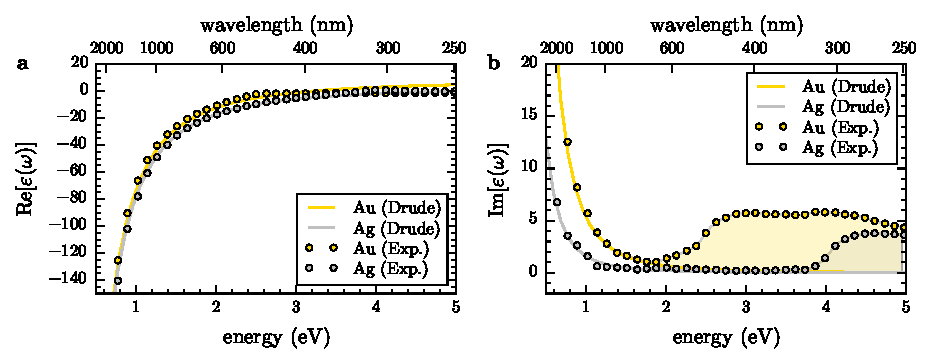
\includegraphics{figures/dielectric_function}
\caption[Plot of the dielectric function, given by the Drude model, for Au and Ag compared with empirical data]{\textbf{Plot of the dielectric function, given by the Drude model, for Au and Ag compared with empirical data.} \dielectric\ is calculated using \eqref{eq:dielectric_function}. The plasma frequency is calculated using \eqref{eq:plasma_frequency}. The parameters of the curves are $n=\SI{5.90e28}{\per\metre\cubed}$, $m=\SI{9.11e-31}{kg}$, $\gamma=1/\tau=1/\SI{1e-14}{s}$ and $\eps_\infty = 8$ for Au and $n=\SI{5.86e28}{\per\metre\cubed}$, $m=\SI{9.11e-31}{kg}$, $\gamma=1/\tau=1/\SI{3e-15}{s}$ and $\eps_\infty = 3$ for Ag. Empirical data (Johnson and Christy, 1972 \cite{johnson1972optical}) is shown for comparison to illustrate the importance of interband transitions. Deviations from the Drude model due to interband transitions are shaded.}
\label{fig:dielectric_function}
\end{figure}

Plotting \eqref{eq:dielectric_function}, along with empirical data, illustrates both why noble metals exhibit high quality visible spectrum (400--\SI{700}{nm}, 1.5--\SI{3}{eV}) plasmonics as well as the failings of the Drude model. Noble metals have $\real{\dielectric}<0$ and small \imag{\dielectric} in the visible region, hence behave very similar to an ideal free electron gas. The Drude model fails at higher energies as interband transitions are not included in the basic model. These transitions increase the absorption ($\propto\imag{\dielectric}$) and are significant for $\lambda < \SI{500}{nm}$ in Au and $\lambda<\SI{300}{nm}$ in Ag. A measure of the quality of a plasmonic material can de determined from its quality factor $\gls{Q} = \left|\real{\eps}/\imag{\eps}\right|$. The high $Q$ of noble metals in the visible regions means they can easily respond to an incident field and screen it, behaving plasmonically. Interband transitions lead to a reduction in \gls{Q} at higher energies therefore preventing good plasmonics.
%Lorentz oscillator terms $m\omega_0i^2x$, where $\omega_0i$ are the natural frequencies of bound electron transitions, can be included in the initial equation of motion to account for such transitions.

\begin{figure}[bt]
\centering
\fontsize{10pt}{1em}\selectfont
\subimport{./figures/}{bulk_charge_displacement.pdf_tex}
\caption[Charge displacement of a free electron gas under an applied field]{\textbf{Charge displacement of a free electron gas under an applied field.} The optical electric field displaces the electrons leaving behind the positive cores. The slab becomes polarised with opposing surface charge densities $\sigma$. The charge oscillations resonate when the field frequency is \omegap.}
\label{fig:bulk_charge_displacement}
\end{figure}

The significance of the plasma frequency \omegap\ in \dielectric\ is that it not only describes a metal-to-dielectric transition but also dictates the frequency of the collective longitudinal mode of oscillation. By substituting \eqref{eq:dielectric_approx} into the dispersion relations for transverse and longitudinal waves it is clear that transverse waves are only supported if $\omega>\omegap$ with dispersion $\omega^2=\omegap[2]+\wvm^2c^2$. However, a collective longitudinal oscillation is allowed at $\omega=\omegap$ since $\dielectric=0$ in the absence of damping. In this case the free electron gas is displaced from the ionic core background a distance \gls{u} due to the applied field to form surface charge densities $\gls{sigma} = \pm neu$. The resulting depolarisation field%
\footnote{Gauss' law $\int \vec{E}\cdot d\vec{A} = Q/\epsfs=\sigma A/\epsfs$, hence $\vec{E}=\sigma/\epsfs$. Alternatively $D=0=\epsfs\vec{E}+\vec{P}$ therefore $\vec{E}=-\vec{P}/\epsfs=-ne\vec{u}/\epsfs$.}
is $\vec{E} = neu/\epsfs$ and the motion of the free electrons are defined by,
\begin{equation}
	nm\ddot{u} = -ne\vec{E} = -\frac{n^2e^2u}{\epsfs}.
\end{equation}
Simplifying this relation leads to,
\begin{equation}
	\ddot{u}+\omegap[2] u=0,
\end{equation}
hence \omegap\ is considered the natural frequency of the system and the electrons resonate when driving at $\omega=\omegap$. This is known as the bulk or \emph{volume plasmon}. Since this is a longitudinal oscillation, however, light cannot couple with a volume plasmon. Experimentally these are measured using \gls{eels}, whereby colliding electrons impart energy and excite a volume plasmon \cite{egerton2011electron}. Observation of optical plasmonic phenomena therefore means that light-matter plasmonics is the result of a different kind of plasmon. % could cite koh2009

\subsection{Surface Plasmons, Surface Plasmon Polaritons and Localised Surface Plasmon Polaritons}
% EELS of LSPs nelayah2007, koh2009, duan2012

\Glspl{sp}, unlike bulk plasmons, are tightly confined to the surface of the metal. As stated previously, light at an interface is not necessarily restricted by the diffraction limit. The maximum magnitude of the wavevector is set by $\wvz=2\pi/\lambda$ with individual components restricted by $\wvm = \sqrt{\wvm_x^2 + \wvm_y^2 + \wvm_z^2}$. Consider \eqref{eq:light_dispersion} in the form,
\begin{equation}
	\wvm_x^2 = \refind^2 \wvz^2 - \wvm_y^2 - \wvm_z^2.
\end{equation}
If a wave propagates freely in all three dimensions then it remains diffraction limited and the propagation constant $\wvm_x < \refind\wvz$. However if one or more of its wavevector components become imaginary ($\wvm_{y,z}^2 < 0$) then it becomes possible that $\wvm_x > \refind\wvz$. This behaviour can occur at an interface, where surface waves take on evanescent character in the $z$-direction whilst propagating in the $xy$ plane.%
\footnote{Evanescent meaning imaginary $\wvm_z$ therefore exponentially decaying amplitude in the $z$-direction.}
By coupling light into surface waves the diffraction limit can be beaten. Waves of frequency $\omega$ can acquire wavelengths many times smaller than their excitation wavelength. The \gls{sp} is one such case of this phenomenon and occurs at metal-dielectric interfaces. % Are there other such cases.
Unlike in the bulk of a metal, electrons displaced by an applied field at the surface of a metal do feel a restoring force with the positive nuclei background. Transverse fields impinging on the metal surface at an angle are then able to manipulate the electron motion. \Glspl{sp} can therefore be manipulated by light as well as by the longitudinal waves needed to excite bulk plasmons.
They also have the ability to form polariton quasiparticles under strong coupling with photons, hence they are  optically excitable under the right conditions.%
\footnote{Polaritons are the name given to quanta or quasiparticles of light-matter interactions. Strong coupling describes the point at which a quasiparticle is no longer distinguishable between it's two constituent components.}
This optical excitation is known as the \gls{spp} and, as a result of it being optically accessible, is one of the most commonly studied plasmonic phenomenons.

\subsubsection{Surface Plasmon Polaritons}

A \gls{spp} is a propagating TM wave confined to the surface of a metal and the bound state between a photon and a \gls{sp}. While confined in two dimensions to the planar boundary between a metal and a dielectric, the \gls{spp} can either propagate or become stationary as a result of interference {\color{red}with itself or other plasmons}. The latter stationary form of the \gls{spp} is similar to the localised surface plasmons described later.

\begin{figure}[bt]
\fontsize{10pt}{1em}\selectfont
\def\svgwidth{0.6\textwidth}
\subimport{./figures/}{spp_diagram.pdf_tex}
\caption[Diagram of a \acrfull{spp}]{\textbf{Diagram of a \acrfull{spp}.} TM surface electron density waves (\acrlongpl{sp}) couple with an evanescent wave originating from an EM wave to form a \gls{spp}. The \gls{spp} remains confined to the interface but can propagate across the surface.}
\label{fig:spp_diagram}
\end{figure}

The \gls{spp} itself is described through its dispersion. As a \gls{tm} wave propagating in the $x$-direction along a metal/dielectric interface its field profile is given by $\vec{E}(\vec{x}) = \vec{E}(z)\e^{i\beta x}$ where $\beta=\wvm_x$ is the propagation constant. The magnetic field in this configuration is then $\vec{H}(\vec{x}) = \vec{H}(y)e^{i\beta x}$. The behaviour of such a wave in \eqref{eq:fourier_wave_equation} is described by,
\begin{subequations}
\begin{align}
	\frac{\partial^2\vec{E}(z)}{\partial z^2} + (\wvz^2\eps - \beta^2)\vec{E} &= 0,\\
	\frac{\partial^2\vec{H}(y)}{\partial y^2} + (\wvz^2\eps - \beta^2)\vec{H} &= 0,
\end{align}
\end{subequations}
which can be solved under the appropriate boundary conditions to yield the properties of a \gls{spp}. Assuming a \gls{tm} wave ($\partial E_y/\partial z = 0$, $\partial H_z/\partial z = 0$), propagating only in the $x$-direction with symmetry in $y$-direction, results in outcomes from \eqref{eq:maxwell3} and \eqref{eq:maxwell4} of,
\begin{subequations}
\begin{align}
	E_x &= -i\frac{1}{\omega\epsfs\eps}\frac{\partial H_y}{\partial z},\\
	E_z &= -\frac{\beta}{\omega\epsfs\eps}H_y.
\end{align}
\end{subequations}
In this instance the \gls{tm} wave equation, and requirement for evanescent decay in the $z$-direction, mean that $H_y = A_d\e^{i\beta x}\e^{\wvm_dz}$ for $z>0$ (in the dielectric) and $H_y = A_m\e^{i\beta x}\e^{\wvm_mz}$ for $z<0$ (in the metal). The components of the electric field can therefore be expressed as,
\begin{subequations}
\begin{align}
	E_x(z) &= iA_d\frac{1}{\omega\epsfs\epsdi}\wvm_d\e^{i\beta x}\e^{-\wvm_dz},\\
	E_z(z) &= -A_d\frac{\beta}{\omega\epsfs\epsdi}\e^{i\beta x}\e^{-\wvm_dz},
\end{align}
\end{subequations}
inside the dielectric and,
\begin{subequations}
\begin{align}
	E_x(z) &= -iA_m\frac{1}{\omega\epsfs\epsmet}\wvm_m\e^{i\beta x}\e^{\wvm_mz},\\
	E_z(z) &= -A_m\frac{\beta}{\omega\epsfs\epsmet}\e^{i\beta x}\e^{\wvm_mz},
\end{align}
\end{subequations}
inside the metal, where $\eps_1=\epsdi$ and $\epsmet=\dielectric$ in the previously used notation. Continuity across the boundary ($z=0$) dictates that $A_d=A_m$ and yields the relation,
\begin{equation}
	\frac{\wvm_2}{\wvm_1} = -\frac{\epsmet}{\epsdi},
	\label{eq:wavevector_ratio}
\end{equation}
hence the ratio between wavevectors inside and outside of the metal depends on the relative change in dielectric constant across the boundary. It is this continuity relation that allows for the existence of \glspl{spp} in the \gls{tm} configuration, unlike for \gls{te} waves for which this result is not possible. To determine the \gls{spp} propagation constant $\beta$ a further relation is needed to fix the wave vectors in a given medium with respect to the dielectric constant. Using the expression for $H_y$ in the wave equation \eqref{eq:fourier_wave_equation} yields a set of relations,
\begin{subequations}
\begin{align}
	\wvm_m^2 = \beta^2 - \wvz^2\epsmet,\\
	\wvm_d^2 = \beta^2 - \wvz^2\epsdi,
\end{align}
\end{subequations}
which, when combined with \eqref{eq:wavevector_ratio}, fully describe the fields around the interface. The propagation constant is then given by,
\begin{equation}
	\beta = \frac{\omega}{c}\sqrt{\frac{\epsdi\dielectric}{\epsdi + \dielectric}}.
	\label{eq:spp_dispersion}
\end{equation}
This is the dispersion relation for a \gls{spp} and describes many of their important properties.

% Dispersion of SPPs
\begin{figure}[bt]
\centering
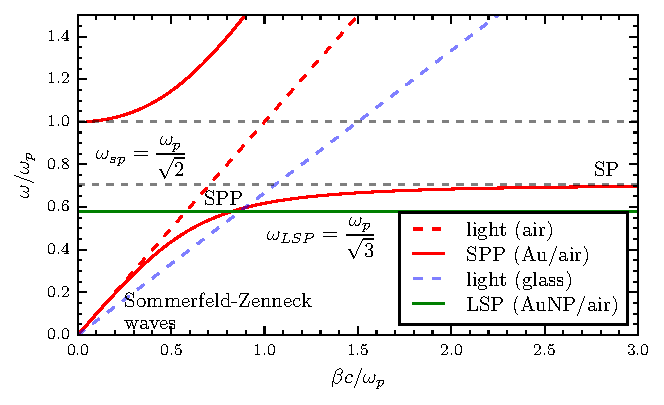
\includegraphics{figures/spp_dispersion}
\caption[Plasmon dispersion relations for the SPP and LSP]{\textbf{Plasmon dispersion relations for the SPP and LSP.} The dashed lines indicate the dispersion of light in both glass and air (vacuum) along with the surface plasmon frequency. SPPs can be described as photon-like or plasmon-like depending on their point of excitation. SPPs excited with large \wvm\ and $\omega\approx\omega_{SPP}$ are considered plasmon-like while SPPs with low \wvm\ are considered more photon-like.}
\label{fig:spp_dispersion}
\end{figure}

% Excitation of SPPs
The \gls{spp} dispersion described by \eqref{eq:spp_dispersion} is shown in \figurename~\ref{fig:spp_dispersion} along with the dispersion of light for both air and glass mediums. From the dispersion curve it is clear that \glspl{spp} cannot couple with light within the same medium as their dispersion curves do not cross. However, light from within a higher refractive index medium such as glass can generate evanescent waves and excite \glspl{spp} on a nearby metal/air interface. This method of coupling photons with surface plasmons, depending on the specific prism arrangement, is known as the Kretschmann (prism-metal-dielectric) or Otto (prism-dielectric-metal) configuration \cite{otto1968, kretschmann1971}. Since a diffraction grating may also impart momentum onto a photon ($\wvm_x \rightarrow \wvm_x + n\pi$) a metallic grating can launch \glspl{spp} along a planar metal-dielectric interface. This phenomenon was first observed in 1902 by Wood, dubbed as Wood's anomaly \cite{wood1902}, and only explained via surface waves many years later \cite{fano1941}.

% Plasmon property: nm-scale wavelength with visible frequency
Closer inspection of the curve highlights one of the major features of a plasmon. While \glspl{spp} retain the frequency of the excitation field, their wavelength is considerably smaller than the diffraction-limited wavelength of light.
% photon-like vs plasmon-like
Depending on where on the curve the \gls{spp} lies it can be considered to be either more photon-like or more plasmon-like. For small $\beta\approx\wvz$ the \gls{spp} is similar to light grazing the interface whereas \glspl{spp} with large \wvm\ become more plasmon-like and their frequency saturates at the surface plasmon frequency,
\begin{equation}
	\omega_{sp} = \frac{\omegap}{\sqrt{1+\epsdi}}.
\end{equation}
At this point the \gls{spp} can be considered electrostatic and becomes a \gls{sp}. To some extent, \glspl{sp} confined to a finite, continuous, non-planar surface, defining a \gls{np}, can be considered to be the basis for a \gls{lsp} {\color{red}or \gls{lspp}}.

\subsubsection{Localised Surface Plasmons}

% Localised Surface Plasmons
\Glspl{lsp} are collective oscillations of conduction electrons confined within a fixed sub-wavelength spatial extent, usually on the surface of a \gls{mnp}. Free electrons are displaced from the nuclei in response to an applied field and form a surface charge distribution, polarising the particle. Coulomb interaction between the poles of the surface charge distribution results in a restoring force within the particle. This gives rise to a natural frequency of oscillation, leading to a \gls{spr} when driven harmonically at the correct frequency.
The particle geometry sets which multipolar surface charge distributions are supported while its material properties and the dielectric properties of the surrounding medium set the restoring force. Each different multipolar charge distribution is therefore considered to be a unique \gls{lsp} mode, identifiable by its \gls{spr} \cite{murray2007}.
This bears some similarity with the slab of free electron gas supporting longitudinal volume plasmons, shown in \figurename~\ref{fig:bulk_charge_displacement}, except that the sub-wavelength geometry modifies the restoring force and allows transverse modes of oscillation. The plasma frequency in \glspl{lsp} is then rescaled by a factor depending on the geometry of each \gls{lsp} mode. %In this sense, \glspl{lsp} can be considered geometrical resonances of the nanostructure. % Not strictly true as geometrical resonances can occur in dielectrics

\begin{figure}[bt]
\centering
\fontsize{10pt}{1em}\selectfont
\def\svgwidth{0.35\textwidth}
\subimport{./figures/}{sphere_plasmon.pdf_tex}
~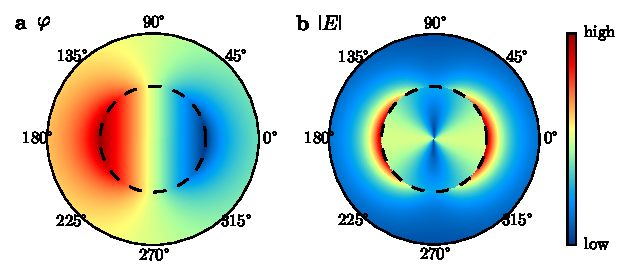
\includegraphics[width=0.59\textwidth]{figures/spherical_np_dipole_lsp}
\caption[A spherical metallic particle in an applied electric field]{\textbf{A spherical metallic particle in an applied electric field.} The sphere is assumed to in the quasistatic regime ($a\ll\lambda$). The aura around the particle indicates the phase of the free electron oscillations in the plasmon. Calculations of (a) the potential and (b) the magnitude of the electric field for a spherical nanoparticle on resonance ($\dielectric=-2\epsdi$).}
\label{fig:sphere_plasmon}
\end{figure}

The simplest form of a \gls{lsp} is the dipole resonance of a spherical \gls{mnp}. Assuming the sphere radius, $\gls{a}\ll\lambda$, the wavelength of light, the particle is considered to be in the quasistatic regime and electrostatics, rather than electrodynamics, is applicable to solve the problem. The electrostatic potential, \gls{potential}, of the system is described by the Laplace equation, $\nabla^2\pot=0$, with a general solution in a spherical geometry of the form,
\begin{equation}
	\pot_{l,m_l}(r,\theta,\phi) = \sum_{l=0}^{l=\infty} \sum_{m_l=-l}^l [ A_lr^l + B_lr^{-(l+1)} ] P_l^m (\cos\theta) \e^{i m_l\phi},
\end{equation}
where \gls{l} is the degree of spherical harmonic and \gls{m_l} its projection, $A_l$ and $B_l$ are constants and $P_l^m(\cos\theta)$ are associated Legendre polynomials. For a sphere of radius $a$ and dielectric function \dielectric\ in a dielectric medium described by \epsdi\ the solution is fixed by the boundary conditions $\pot_{\mathrm{out}}\rightarrow-E_0z$ as $r\rightarrow\infty$ and $\left.\nabla\pot_{in}(r)\right|_{r=a}=\left.\nabla\pot_{out}(r)\right|_{r=a}$. This reduces to a solution \cite{jackson1999classical},
\begin{equation}
	\pot =
	\begin{dcases}
	-\frac{3\epsdi}{\dielectric + 2\epsdi} \vec{E_0}\cdot\vec{r} & r \leq a\text{ (inside)}, \\
	\left(-1 + \frac{\dielectric - \epsdi}{\dielectric + 2\epsdi} \frac{a^3}{r^3}\right) \vec{E_0}\cdot\vec{r} & r > a\text{ (outside)}.
	\end{dcases}
\end{equation}
%\begin{subequations}
%\begin{align}
%\pot_{\mathrm{in}} &= -\frac{3\epsdi}{\dielectric + 2\epsdi} \vec{E_0}\cdot\vec{r}, \\
%\pot_{\mathrm{out}} &= \left(-1 + \frac{\dielectric - \epsdi}{\dielectric + 2\epsdi} \frac{a^3}{r^3}\right) \vec{E_0}\cdot\vec{r}.
%\end{align}
%\end{subequations}
For a metal sphere the potential describes an induced dipolar surface charge distribution, as plotted in \figurename~\ref{fig:sphere_plasmon}a. The description is simplified by defining the dipole moment as,
\begin{equation}
	\vec{p} = \epsfs\epsdi\alpha\vec{E_0} = 4\pi\epsfs\epsdi a^3 \frac{\dielectric - \epsdi}{\dielectric + 2\epsdi} \vec{E_0},
\end{equation}
where the polarisability, \gls{alpha}, incorporates the frequency dependent behaviour and is defined as,
\begin{equation}
	\alpha(\omega) = 4\pi a^2 \frac{\dielectric - \epsdi}{\dielectric + 2\epsdi}.
	\label{eq:polarisability}
\end{equation}
The outside potential is then expressed as,
\begin{equation}
	%\Phi_{out} = -E_0r\cos{\theta} + \frac{\vec{p}\cdot\vec{r}}{4\pi\varepsilon_0\varepsilon_m r^3}.
	\pot_{out} = -\vec{E_0}\cdot\vec{r} + \frac{\vec{p}\cdot\vec{r}}{4\pi\epsfs\epsdi r^3}.
\end{equation}
The potential of the system is simply the potential of a dipole superimposed onto the incident field. The electric field inside and outside of the sphere is calculated using $\vec{E}=-\nabla\pot$, resulting in,
\begin{equation}
	\vec{E} =
	\begin{dcases}
	\frac{3\epsdi}{\dielectric+2\epsdi} \vec{E_0} & r \leq a\text{ (inside)}, \\
	\vec{E_0} + \frac{3\vec{n}(\vec{n}\cdot\vec{p}) - \vec{p}}{4\pi\epsfs\epsdi}\frac{1}{r^3} & r > a\text{ (outside)},
	\end{dcases}
	\label{eq:E_out}
\end{equation}
%\begin{subequations}
%\begin{align}
%\vec{E_{in}} &= \frac{3\epsdi}{\dielectric+2\epsdi} \vec{E_0}, \\
%\vec{E_{out}} &= \vec{E_0} + \frac{3\vec{n}(\vec{n}\cdot\vec{p}) - \vec{p}}{4\pi\epsfs\epsdi}\frac{1}{r^3}, \label{eq:E_out}
%\end{align}
%\end{subequations}
where $\vec{n}=\vec{r}/r$ is the unit vector. As with the potential, the electric field is the superposition of the incident field with the field emitted from a point dipole, shown in \figurename~\ref{fig:sphere_plasmon}b.

It is assumed from its sub-wavelength size that electrons in the sphere respond instantaneously to the incident field and phase retardation is ignored (quasistatic approximation). Under this assumption the electrostatic result is simply multiplied with a harmonic time dependence to describe electrodynamic behaviour. Therefore, when illuminated by a plane wave $\vec{E_0}\e^{i\omega t}$ the induced dipole moment oscillates like $\vec{p}\e^{i\omega t}$. In this sense the coherent oscillation of free electrons in the sphere is considered to be an oscillating point dipole source given by $\vec{p}\e^{i\omega t}=\epsfs\epsdi\alpha\vec{E_0}\e^{i\omega t}$. The physical behaviour of the electrons in the sphere, described using the dielectric function \dielectric\ , is then simply incorporated into $\alpha(\omega)$, at which point its frequency dependence becomes important.

For a good metal $\real{\dielectric}<0$ and the denominator in \eqref{eq:polarisability} undergoes resonance whereby $\alpha\rightarrow-\infty$ when $\dielectric+2\epsdi\rightarrow0$. Resonance therefore occurs at the Fr\"{o}hlich condition when,
\begin{equation}
\real{\dielectric} = -2\epsdi. \label{eq:frohlich}
\end{equation}
Resonant excitation of the induced oscillating dipole moment corresponds to excitation of a collective oscillation of conduction electrons on the surface of the sphere - the dipolar \gls{lsp}. It's strength in realistic metals is restricted by damping of the electron motion leading to a Lorentzian-shaped resonance band - the dipolar \gls{spr}. As seen in \eqref{eq:E_out}, the field from the induced dipole moment of the plasmon is superimposed onto the incident field leading to a resonant near-field enhancement, both inside and outside the surface of the sphere. This is one of the fundamental properties of the plasmon, and one that is most exploited in sensing and sensor developments.

Under the Drude model, with \dielectric\ given by \eqref{eq:dielectric_function}, the Fr\"{o}hlich condition is satisfied when,
\begin{equation}
\omega_{lsp} = \frac{\omegap}{\sqrt{1+2\epsdi}},
\end{equation}
which evaluates to $\omega = \omegap/\sqrt{3}$ for a \gls{mnp} in vacuum. As can be seen in \figurename~\ref{fig:spp_dispersion}, the flat dispersion of a \gls{lsp} mode means it crosses the light line at a single point. Light of the correct frequency therefore readily couples with \glspl{lsp} without the need for \gls{spp} momentum matching mechanisms.
% Spherical harmonics
In general, the optical spectrum of a \gls{mnp} can contain a number of multipolar plasmon modes {\color{red}other than the dipole mode} for which the resonant frequencies are given by,
\begin{equation}
\omega_l = \omegap\sqrt{\frac{l}{\epsdi(l+1)+1}},
\end{equation}
where the degree of spherical harmonics $l$ denote the charge distribution and denoted mode order ($l=1$ for dipole, $l=2$ for quadrupole, etc.). However, these modes only exist outside of the quasistatic regime in larger \glspl{mnp} or more complex geometries.
% Link with noble metals
For plasmonically-active nobles metals, such as Au and Ag, the fundamental $l=1$ mode occurs in the visible spectrum ($\lambda=\SI{520}{nm}$ for Au and $\lambda=\SI{360}{nm}$ for Ag), leading to them often being the plasmonic metal of choice.
% geometry dependence
Additionally, since the polarisability changes with \gls{np} geometry, changes from a spherical shape lead to tuning of the \glspl{spr} across the visible spectrum. This geometrical dependence is well known and has been measured experimentally on a number of occasions \cite{mock2002, kuwata2003}.

As with any oscillating charge distribution, energy is both absorbed and emitted from the plasmon. The oscillating charge has the ability to scatter the incident planar field into spherical waves. The excitation of a resonant dipolar oscillation means that the scattering is also resonantly enhanced. The balance between the absorbance and the scattering from a \gls{mnp} is dictated by its size. The absorbance and scattering cross sections are given by \cite{bohren2008absorption},
\begin{subequations}
\begin{align}
\gls{sigma_scat} &= \frac{\wvm^4}{6\pi} |\alpha|^2 = \frac{8\pi}{3}\wvm^4a^6 \left| \frac{\dielectric - \epsdi}{\dielectric + 2\epsdi} \right|^2, \\
\gls{sigma_abs} &= \wvm\imag{\alpha} = 4\pi \wvm a^3 \imag{ \frac{\dielectric - \epsdi}{\dielectric + 2\epsdi} }.
\end{align}
\end{subequations}
The extinction cross section, commonly used in spectroscopy, can be calculated using $\gls{sigma_ext}=\sigma_{\mathrm{scat}}+\sigma_{\mathrm{abs}}$. Since they depend on $\alpha$ the size of the cross section, i.e. the spatial extent over which light can interact with the \gls{mnp}, is increased on resonance. This is why \glspl{mnp} appear strongly coloured and much larger in optical microscopy than they actually are. The absorbance and scattering cross sections scale as $a^3$ and $a^6$, respectively, hence larger particles scatter more than they absorb whereas absorption dominates in smaller particles.

From the cross-sections the relationship between the \gls{lsp} near-field and the far-field is made clearer. On resonance with the dipolar \gls{lsp}, both cross sections are enhanced by the polarisability resonance from \orderof{$a\sim\SI{50}{nm}$} to \orderof{\SI{500}{nm}}. The increased size of the cross-section is comparable to the wavelength of light meaning \glspl{lsp} efficiently couple with photons in the far-field.%
\footnote{Consider that $\sigma_{\mathrm{scat}}$ for a AuNP is enhanced $100\times$ on resonance, meaning it's area cross-section is $\sqrt{100/\pi}= 6\times$ wider than it's radius, hence why a \SI{50}{nm} AuNP looks like a \SI{300}{nm} green sphere when imaged.}
The \gls{lsp} mediates energy transfer between the near-field and the far-field and acts to match the electromagnetic modes of nanoscale absorbers/emitters, such as phonons (Raman) and radiative energy levels (quantum emitters, fluorescence), with those of a diffraction-limited photonic mode via an oscillating charge density \cite{berweger2012}. A plasmonic \gls{np} is often therefore described as an \textit{optical antenna} in a similar manner to a device that converts between radio waves and an electrical current is named a radio antenna. \Gls{lsp} modes which readily couple with the far-field are then sometimes referred to as \emph{antenna modes} and become important when designing resonant structures for specific sensing applications.

\begin{figure}[bt]
\centering
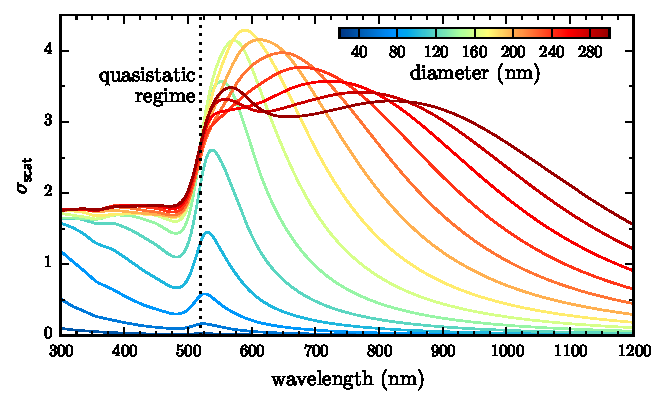
\includegraphics{figures/mie_scattering}
\caption[Mie scattering {\color{red}efficiencies/cross-sections} for AuNPs of increasing diameter]{\textbf{Mie scattering {\color{red}efficiencies/cross-sections} for AuNPs of increasing diameter.} The \SI{520}{nm} resonance position of the dipolar LSP mode of a AuNP in the quasistatic approximation is indicated by the dotted line. The resonance stays at \SI{520}{nm} until $d>\SI{80}{nm}$ then redshifts. The emergence of higher order modes following a similar behaviour is seen once $d>\SI{100}{nm}$.}
\label{fig:mie_scattering}
\end{figure}

Whilst the quasistatic approach is useful to first demonstrate the enhancing capabilities of a \gls{mnp}, the description breaks down once the size of the particle becomes more comparable to the excitation wavelength. Retardation effects between the field and the electrons mean that phase differences between the charge oscillations and the incident field become important. At this point Mie theory (electrodynamics) is required to describe the spectral response of spherical \glspl{mnp} \cite{mie1908}. Mie theory provides a more general description of the optical response of spherical \glspl{mnp}. Using this approach the spectra of a \gls{mnp} can be decomposed into superimposed multipoles, alluding to the existence of higher order \gls{lsp} modes in larger \glspl{mnp}. The spectral response of spherical AuNPs of varying sizes is shown in \figurename~\ref{fig:mie_scattering}, demonstrating the redshift and broadening of lower order modes with increasing particle size and the excitation of higher order modes.
%Furthermore, from \figurename~\ref{fig:mie_scattering}, though the scattering cross-section given by Mie theory is significantly less than from the electrostatic result, the enhanced cross-section still remains relatively large in comparison. This again explains why diffraction-limited light efficiently couples well with metallic nanostructures. The increased cross sections acts as a means of mode-matching the similarly sized incident fields with the nanoscale geometry.

\subsubsection{Geometrical Influences on Localised Surface Plasmon Resonances}

As previously stated, the \gls{lsp} is a geometrical resonance and exists primarily due to the interplay between the driving field inducing oscillations in the mobile electrons and the resulting restoring force acting between the positive ionic core background and the accumulation of conduction electrons at the surface. While the surface charge oscillation directly correlates to the driving field the restoring force, incorporated into the polarisability, is geometry dependent. The \glspl{spr} of a single particle are therefore very geometry dependent \cite{krenn2000, mock2002, kuwata2003}.
The larger the separation between opposing surface charge poles in the antenna, the weaker the restoring force. As seen with Mie theory, a larger particle with a smaller restoring force has a lower energy resonance. The same can be said if the particle geometry is elongated (a nanoellipsoid or nanorod). Within the quasistatic regime, the polarisability of an ellipsoidal \gls{mnp} is adjusted by inserting a geometrical correction, leading to the redefinition,
\begin{equation}
\alpha_i(\omega) = 4\pi a_1a_2a_3\frac{\dielectric-\epsdi}{3\epsdi+3L_i(\dielectric-\epsdi)},
\end{equation}
where $i$ is the index of each anisotropic axis with a geometrical factor,
\begin{equation}
L_i = \frac{a_1a_2a_3}{2}\int_0^\infty \frac{dq}{(a_i^2+q)\sqrt{(q+a_1^2)(q+a_2^2)(q+a_3^2)}}.
\end{equation}
The resonance condition along each axis is then changed to,
\begin{equation}
\real{\dielectric} = -\frac{1 - L_i}{L_i}\epsdi.
\end{equation}
By decreasing the geometrical factor the resonance condition decreases from $-2\epsdi$, corresponding to a decreased resonant frequency and a redshifted \gls{spr}. The longer the particle is, the larger the redshift until the particle is large enough to no longer be considered plasmonic. Continual separation of the poles inevitably weakens the restoring force to the point that each lowest-order antenna \gls{spr} no longer exists.
%For the case where there is no restoring force electrons respond directly in anti-phase to the incident field (Drude model) until the field oscillates too quickly for the electrons to follow, i.e. $\omega>\omegap$. Under these conditions there is no resonance.

By utilising the particle material, geometry and polarisation anisotropy to tune the plasmon resonance, the resonant wavelength band can be shifted across the entire UV--NIR spectrum to tailor individual applications. The limitation to this technique is the relatively small field enhancement that a single particle can provide.
% Lead into plasmon coupling
An alternative approach to exploiting \glspl{lsp} is therefore to couple the fields of many plasmons together. Through coupling the confined fields in the gaps between \glspl{mnp} can be enhanced by many more orders of magnitudes.

\end{document}